\section{ИССЛЕДОВАНИЕ РАБОТЫ ДВОИЧНО-ДЕСЯТИЧНОГО СЧЕТЧИКА
}

Микросхема имеет два входа асинхронного сброса R1 и R2, объединенные логической функцией «И». В счетчике предусмотрена возможность предварительной асинхронной установки двоичного кода 1001. Для
этого используются входы S1 и S2, также объединенные логической функцией «И». В режиме счета по срезу каждого тактового импульса, поступающего на вход С0, происходит увеличение выходного кода счетчика на
единицу
\begin{figure}[H]
	\centering
	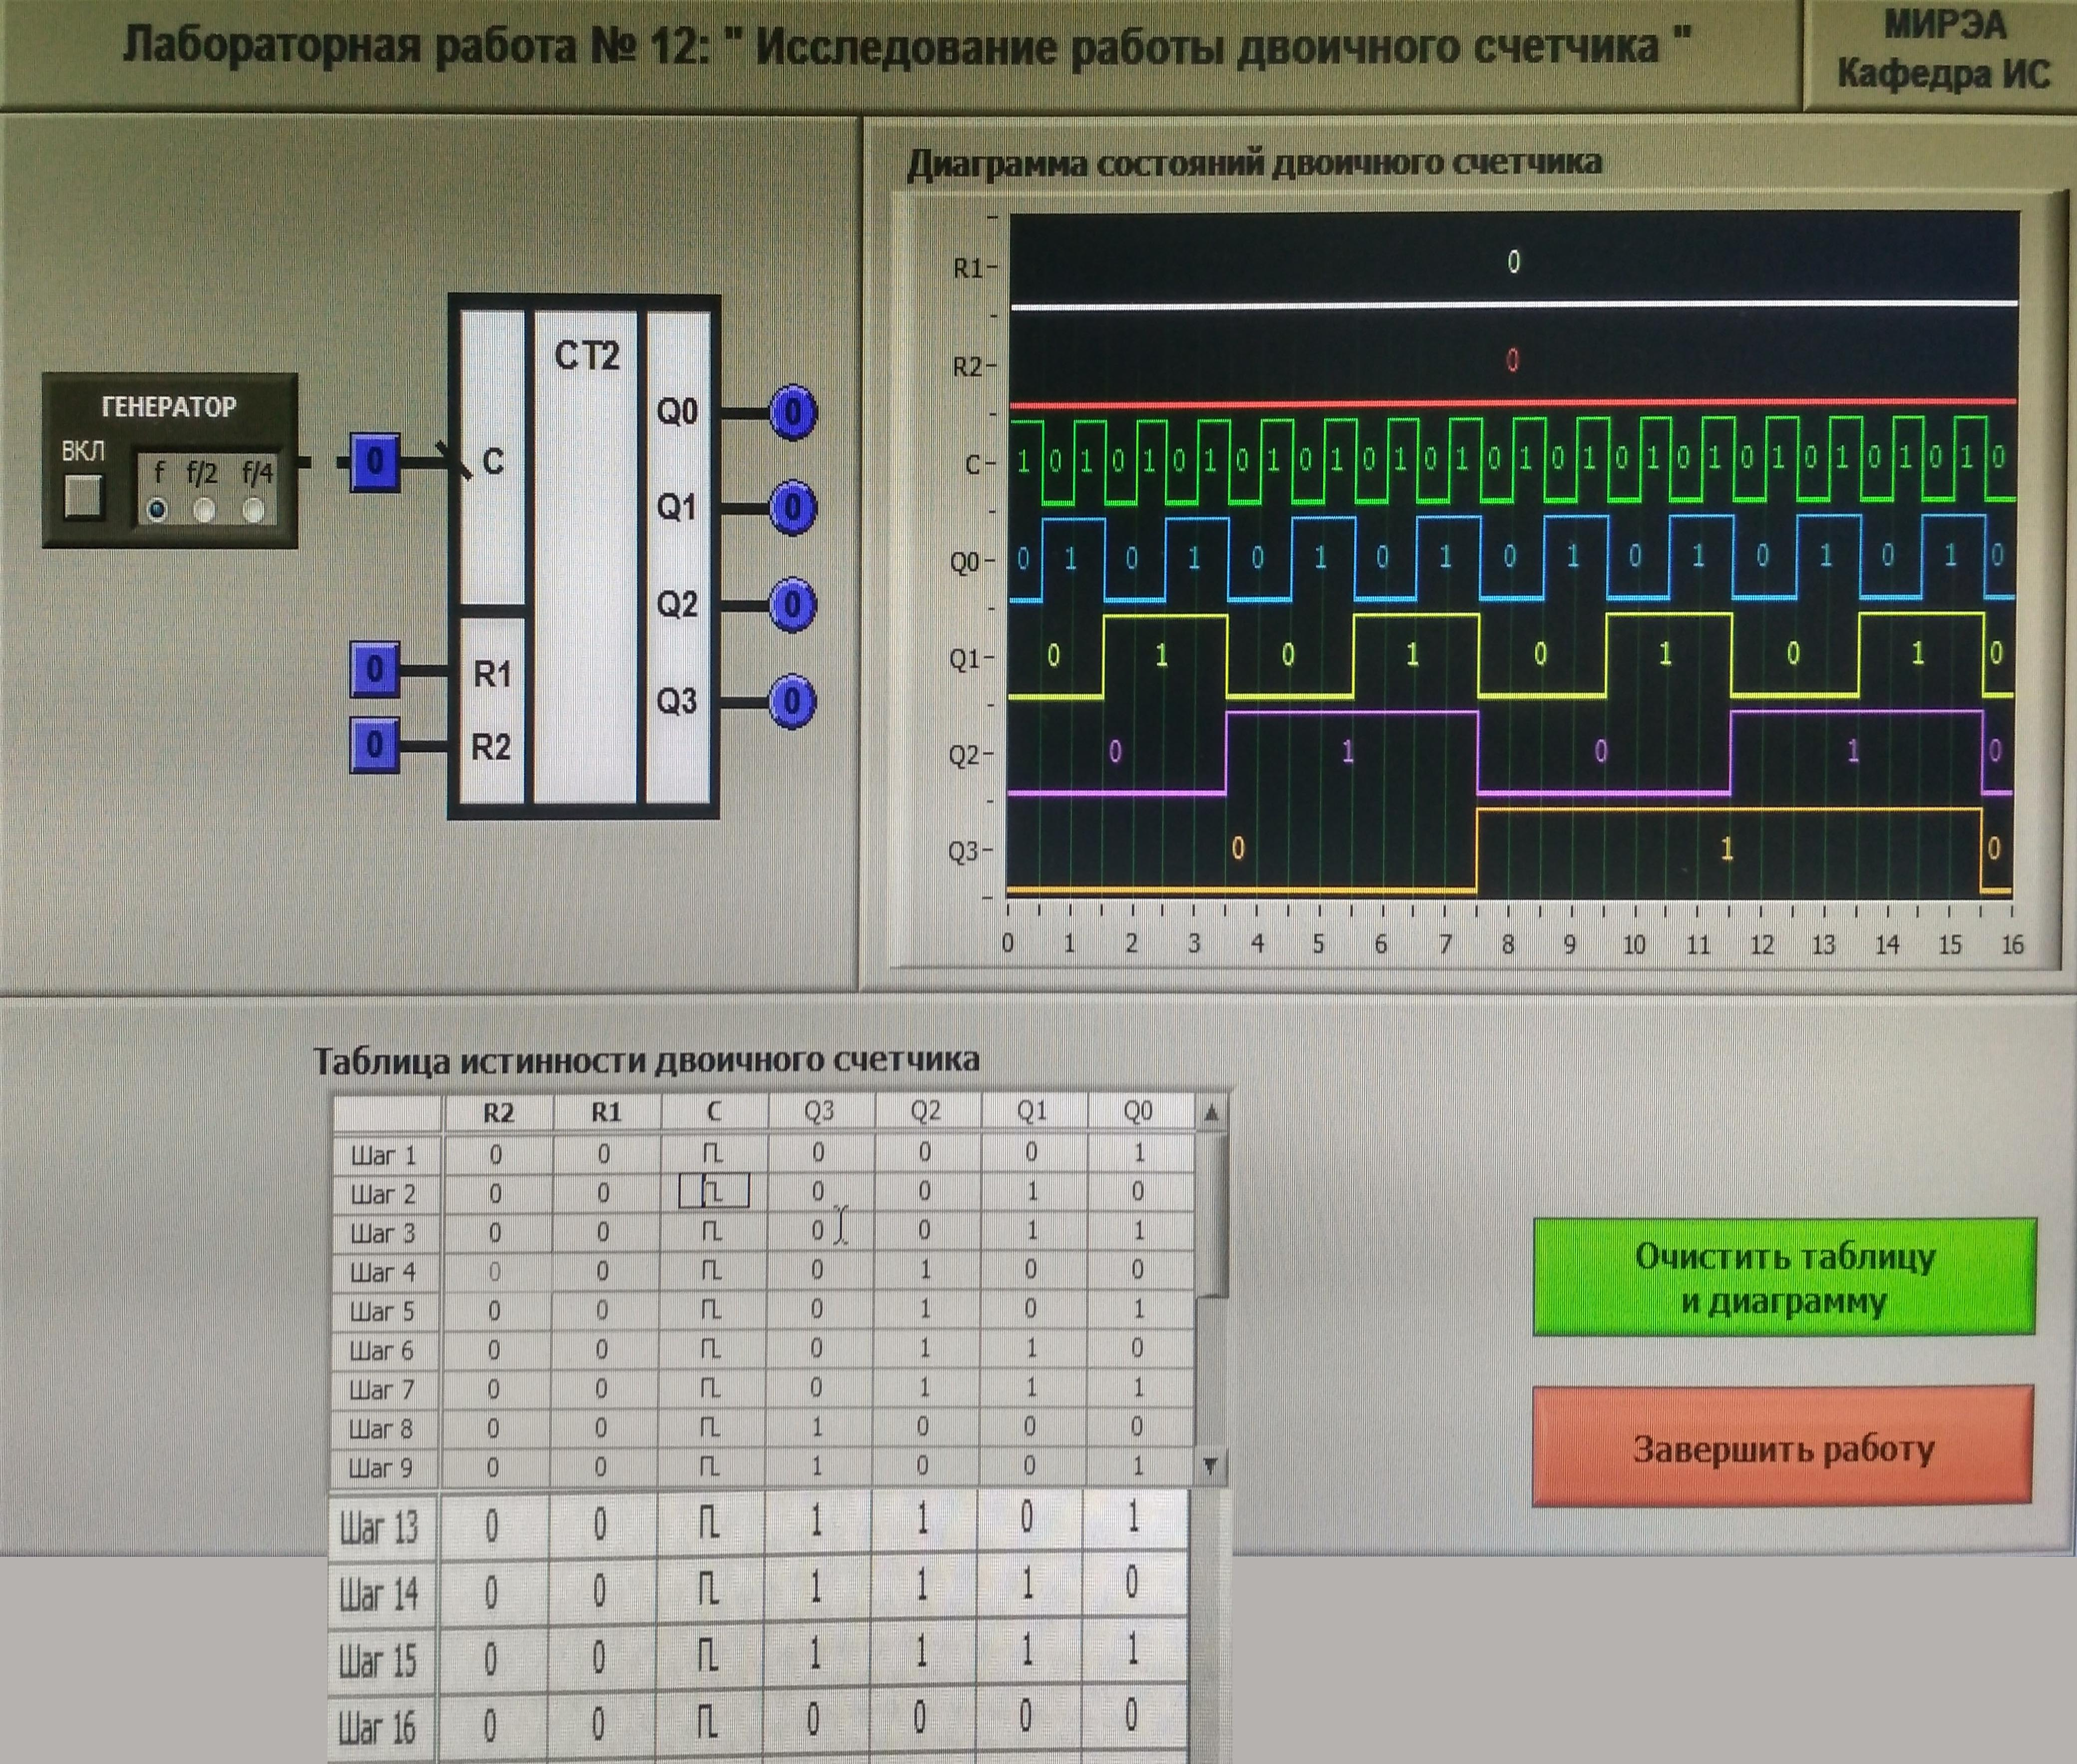
\includegraphics[width=0.95\linewidth]{imgs/13/1.jpg}
	\caption{Исследование двоично-десятичного счетчика в статическом режиме}
	\label{fig:13_1}
\end{figure}

\begin{figure}[H]
	\centering
	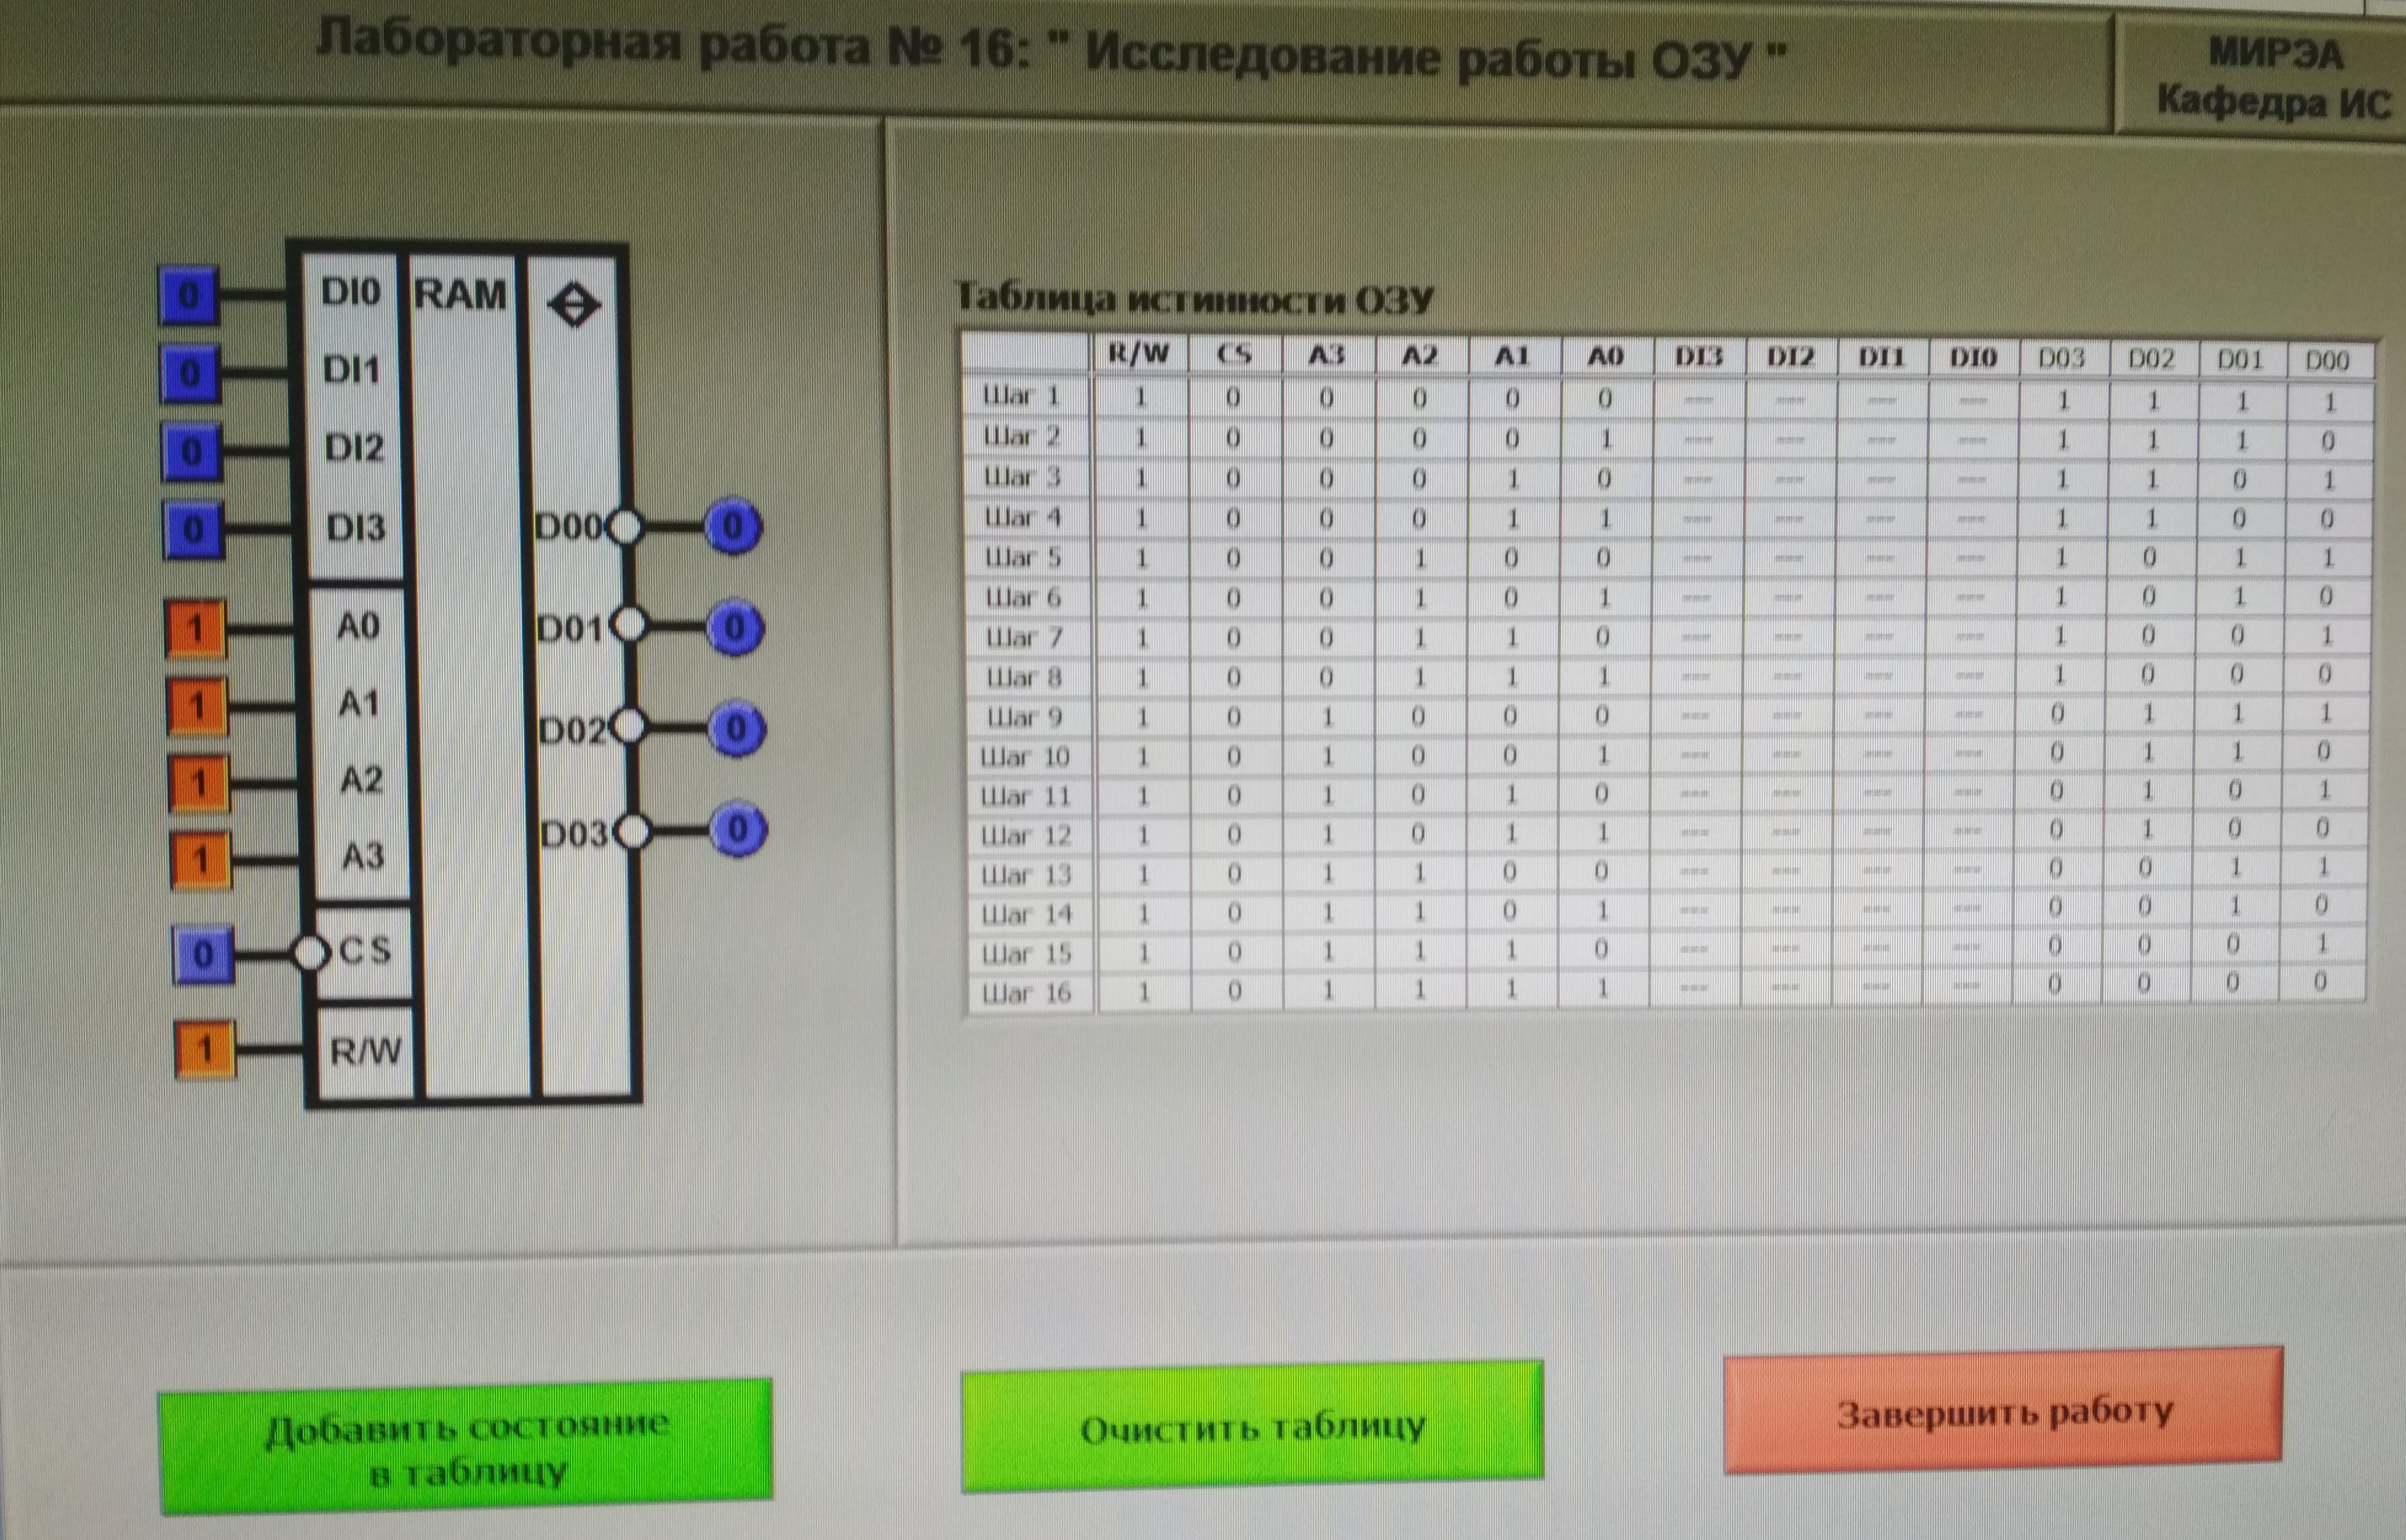
\includegraphics[width=0.95\linewidth]{imgs/13/2.jpg}
	\caption{Исследование двоичного счетчика в динамическом режиме}
	\label{fig:13_2}
\end{figure}

\begin{figure}[H]
	\centering
	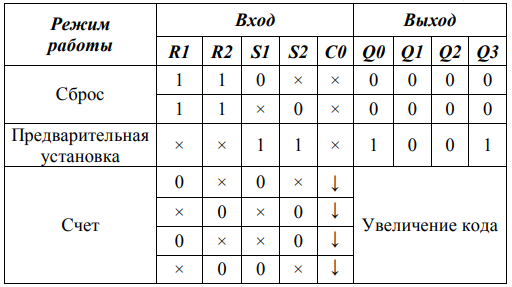
\includegraphics[width=0.85\linewidth]{imgs/13/13_tab}
	\caption{Режим работы сумматора}
	\label{fig:13_tab}
\end{figure}

Элемент SN74LS90 - Low-Voltage BiCMOS Technology

Характеристики:

\begin{figure}[H]
	\centering
	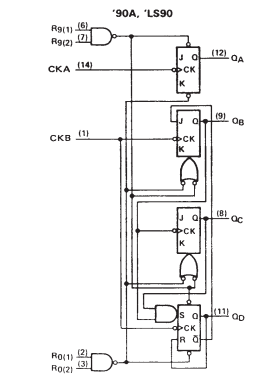
\includegraphics[width=0.55\linewidth]{imgs/13/13_sh}
	\caption{Схема}
	\label{fig:13_sh}
\end{figure}

\begin{figure}[H]
	\centering
	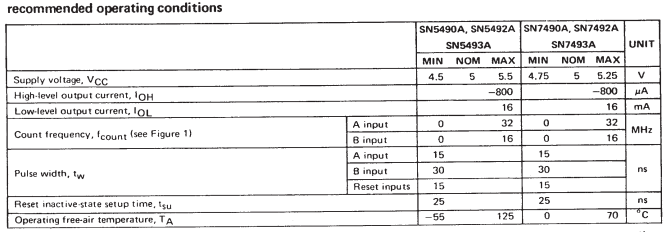
\includegraphics[width=0.95\linewidth]{imgs/13/13_rec}
	\caption{Рекомендуемые параметры}
	\label{fig:13_rec}
\end{figure}

\begin{figure}[H]
	\centering
	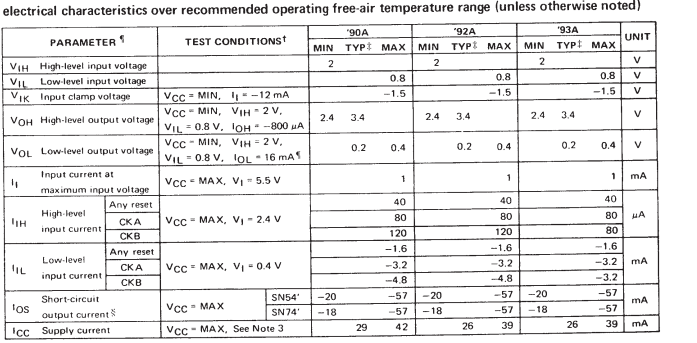
\includegraphics[width=0.95\linewidth]{imgs/13/13_ch}
	\caption{Электрические характеристики}
	\label{fig:13_ch}
\end{figure}

\begin{figure}[H]
	\centering
	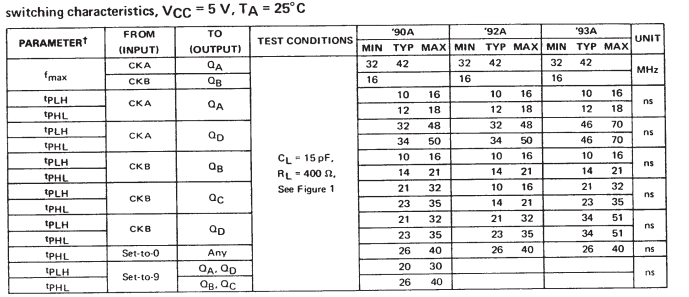
\includegraphics[width=0.95\linewidth]{imgs/13/13_switch}
	\caption{Коммутационные характеристики}
	\label{fig:13_switch}
\end{figure}
